% ==============================================================
% VLM Embodied Agent on TIAGo — ECAI 2026 Preprint
% Presentation — LISSI Laboratory, UPEC
% Author: Abderrahmene Amar Benhamlaoui, Attal, Chibani, Amirat
% ==============================================================
\documentclass[aspectratio=169, 10pt]{beamer}

\usetheme{Madrid}
\usecolortheme{whale}

% ---------- Packages first ----------
\usepackage[utf8]{inputenc}
\usepackage[T1]{fontenc}
\usepackage{lmodern}
\usepackage{xcolor}
\usepackage{tikz}
\usetikzlibrary{shapes,arrows.meta,positioning,calc}
\usepackage{booktabs}
\usepackage{graphicx}
\usepackage{amsmath}

% ---------- Base colors ----------
\definecolor{upecred}{RGB}{206, 32, 41}
\definecolor{upecdark}{RGB}{35, 31, 32}
\definecolor{upecgray}{RGB}{100, 100, 100}
\definecolor{lightgray}{RGB}{245, 245, 245}
\definecolor{softblue}{RGB}{44, 82, 130}
\definecolor{softgreen}{RGB}{39, 124, 72}
\definecolor{navyblue}{RGB}{0, 70, 127}

% ---------- Pre-mixed colors (NO ! inside TikZ options) ----------
\colorlet{cRed8}{upecred!8}
\colorlet{cRed10}{upecred!10}
\colorlet{cRed12}{upecred!12}
\colorlet{cRed15}{upecred!15}
\colorlet{cRed50}{upecred!50}
\colorlet{cNavy8}{navyblue!8}
\colorlet{cNavy10}{navyblue!10}
\colorlet{cNavy12}{navyblue!12}
\colorlet{cNavy18}{navyblue!18}
\colorlet{cBlue10}{softblue!10}
\colorlet{cBlue12}{softblue!12}
\colorlet{cGreen8}{softgreen!8}
\colorlet{cGreen10}{softgreen!10}
\colorlet{cGreen12}{softgreen!12}
\colorlet{cGreen80}{softgreen!80!black}
\colorlet{cDark8}{upecdark!8}
\colorlet{cDark10}{upecdark!10}
\colorlet{cDark15}{upecdark!15}
\colorlet{cDark20}{upecdark!20}
\colorlet{cGray10}{gray!10}
\colorlet{cGray15}{gray!15}

% ---------- Beamer colors ----------
\setbeamercolor{structure}{fg=upecred}
\setbeamercolor{palette primary}{bg=upecdark, fg=white}
\setbeamercolor{palette secondary}{bg=upecred, fg=white}
\setbeamercolor{palette tertiary}{bg=upecred, fg=white}
\setbeamercolor{palette quaternary}{bg=upecdark, fg=white}
\setbeamercolor{frametitle}{bg=upecdark, fg=white}
\setbeamercolor{block title}{bg=upecdark, fg=white}
\setbeamercolor{block body}{bg=lightgray}
\setbeamercolor{block title alerted}{bg=upecred, fg=white}
\setbeamercolor{block body alerted}{bg=cRed8}
\setbeamercolor{block title example}{bg=softgreen, fg=white}
\setbeamercolor{block body example}{bg=cGreen8}
\setbeamercolor{item}{fg=upecred}

% ---------- TikZ styles ----------
\tikzset{
  pbox/.style={draw,rounded corners=3pt,align=center,font=\small,
               text width=4.5cm,minimum height=0.65cm},
  arr/.style={-{Stealth[length=2.5mm]},thick},
}

% ---------- Title ----------
\title[VLM Embodied Agent on TIAGo]{%
  \textbf{End-to-End VLM + Neuro-Symbolic State Manager\\
  for Robot Manipulation on TIAGo}}
\subtitle{System Integration Demonstration — ECAI 2026 Preprint}
\author[A.\,Benhamlaoui \textit{et al.}]{%
  \textbf{Abderrahmene Amar Benhamlaoui},\enspace
  F.\,Attal,\enspace I.\,Kenai,\enspace A.\,Chibani,\enspace Y.\,Amirat}
\institute[LISSI -- UPEC]{%
  LISSI Laboratory (EA\,3956)\\
  Universit\'{e} Paris-Est Cr\'{e}teil (UPEC), France}
\date{2026}

\logo{
\includegraphics[height=0.65cm]{figs/UPEC-logo.svg.png}}
\setbeamertemplate{navigation symbols}{}

\setbeamertemplate{footline}{%
  \leavevmode\hbox{%
    \begin{beamercolorbox}[wd=.33\paperwidth,ht=2.25ex,dp=1ex,center]{palette primary}
      \usebeamerfont{author in head/foot}\insertshortauthor
    \end{beamercolorbox}%
    \begin{beamercolorbox}[wd=.44\paperwidth,ht=2.25ex,dp=1ex,center]{palette secondary}
      \usebeamerfont{title in head/foot}\insertshorttitle
    \end{beamercolorbox}%
    \begin{beamercolorbox}[wd=.23\paperwidth,ht=2.25ex,dp=1ex,right]{palette tertiary}
      \insertframenumber{}/\inserttotalframenumber\hspace*{1.5ex}
    \end{beamercolorbox}%
  }\vskip0pt}

% =====================================================================
\begin{document}

% -------------------- TITLE --------------------
{
\setbeamertemplate{footline}{}
\begin{frame}
  \begin{columns}[c]
    \begin{column}{0.18\textwidth}
      \centering
\includegraphics[width=\linewidth]{figs/UPEC-logo.svg.png}
    \end{column}
    \begin{column}{0.80\textwidth}
      {\small\color{upecgray}
        LISSI Laboratory (EA\,3956) ---
        Universit\'{e} Paris-Est Cr\'{e}teil}\\[0.35cm]
      {\large\bfseries\color{upecdark}
        End-to-End Integration of a VLM\\
        with a Neuro-Symbolic State Manager\\
        for Embodied Robot Manipulation on TIAGo}\\[0.2cm]
      {\normalsize\color{upecred}
        System Integration Demonstration}\\[0.35cm]
      {\small
        \textbf{Abderrahmene Amar Benhamlaoui},\enspace
        Ferhat Attal,\enspace
        Abdelghani Chibani,\enspace
        Yacine Amirat\\[0.1cm]
        ECAI 2026 Preprint \textbullet\ LISSI Lab, UPEC, France}
    \end{column}
  \end{columns}
  \vspace{0.25cm}
  \begin{center}
    \textcolor{upecred}{\rule{0.6\textwidth}{1.2pt}}\\[0.1cm]
    {\scriptsize\color{upecgray}
      Embodied Agent \textbullet\ VLA \textbullet\
      Neuro-Symbolic \textbullet\ Open-Vocabulary Perception \textbullet\ TIAGo}
  \end{center}
\end{frame}
}

% -------------------- OUTLINE --------------------
\begin{frame}{Outline}
  \tableofcontents
\end{frame}

% =====================================================================
\section{Motivation}
% =====================================================================

\begin{frame}{Building an Embodied Robot Agent}
  \begin{columns}[T]
    \begin{column}{0.54\textwidth}
      \textbf{Goal:} a robot that listens, sees, decides, and acts ---
      in a \textbf{closed loop}, without retraining.

      \vspace{0.4em}
      \textbf{Three gaps in existing systems:}
      \begin{enumerate}\small
        \item \textbf{Fixed-vocabulary perception}\\
              YOLO needs retraining for every new object class
        \item \textbf{Static world models}\\
              RDF/OWL graphs built offline; cannot update after manipulation
        \item \textbf{No GPU-free full loop}\\
              No open system closes voice$\to$grasp$\to$handover
              on a real mobile robot without a GPU
      \end{enumerate}

      \vspace{0.3em}
      \begin{alertblock}{Our answer}
        \small
        Cloud VLM as cognitive core + live symbolic state manager,\\
        deployed on a real \textbf{TIAGo} at LISSI Lab, UPEC.
      \end{alertblock}
    \end{column}

    \begin{column}{0.42\textwidth}
      \centering
      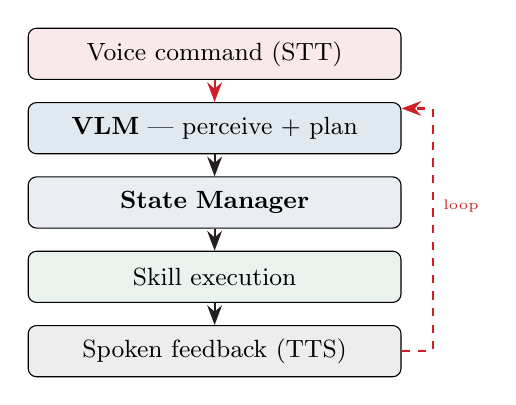
\begin{tikzpicture}[node distance=0.28cm]
        \node[pbox,fill=cRed10] (v) {Voice command (STT)};
        \node[pbox,fill=cNavy12,below=of v] (vlm) {\textbf{VLM} --- perceive + plan};
        \node[pbox,fill=cBlue10,below=of vlm] (sm) {\textbf{State Manager}};
        \node[pbox,fill=cGreen10,below=of sm] (sk) {Skill execution};
        \node[pbox,fill=cDark8,below=of sk] (fb) {Spoken feedback (TTS)};
        \draw[arr,draw=upecred] (v)--(vlm);
        \draw[arr,draw=upecdark] (vlm)--(sm);
        \draw[arr,draw=upecdark] (sm)--(sk);
        \draw[arr,draw=upecdark] (sk)--(fb);
        \draw[arr,draw=upecred,dashed]
          (fb.east)--++(0.4,0)|-([yshift=0.25cm]vlm.east)
          node[pos=0.3,right,font=\tiny,color=upecred]{loop};
      \end{tikzpicture}
    \end{column}
  \end{columns}
\end{frame}

% =====================================================================
\section{System Architecture}
% =====================================================================

\begin{frame}{Three-Layer Neuro-Symbolic Architecture}
  \vspace{-0.2em}
  {\scriptsize
  \textbf{L1 Neural} (VLM: perceive + plan)\enspace$\longrightarrow$\enspace
  \textbf{L2 Symbolic} (StateManager: scene ontology)\enspace$\longrightarrow$\enspace
  \textbf{L3 Action} (Skill Library + ROS/MoveIt)\enspace$\longrightarrow$\enspace
  \textbf{TIAGo hardware}}
  \vspace{0.3em}
  \begin{center}
    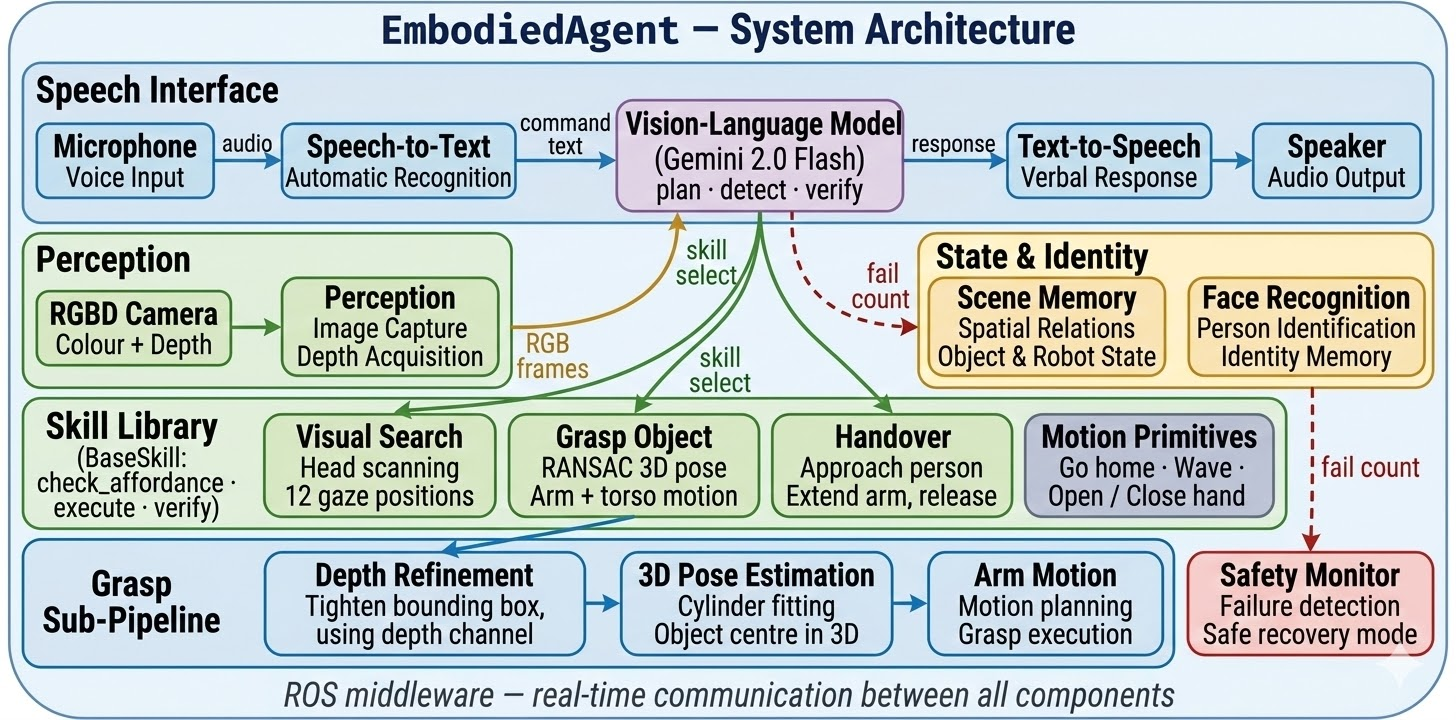
\includegraphics[width=\textwidth,height=0.72\textheight,keepaspectratio]{unnamed.jpg}
  \end{center}
\end{frame}

\begin{frame}{Seven Skills in the Action Library}
  \begin{columns}[T]
    \begin{column}{0.50\textwidth}
      \begin{block}{Complete skill repertoire}
        \small
        \renewcommand{\arraystretch}{1.2}
        \begin{tabular}{ll}
          \toprule
          \textbf{Skill} & \textbf{Purpose}\\
          \midrule
          \texttt{search\_with\_head}   & Scan 12 positions for target\\
          \texttt{grab\_bottle}         & RGBD-guided grasp\\
          \texttt{handover\_to\_person} & Arm extension + delivery\\
          \texttt{wave}                 & Social gesture\\
          \texttt{go\_home}             & Safe arm retraction\\
          \texttt{open\_hand}           & Open gripper\\
          \texttt{close\_hand}          & Close gripper\\
          \bottomrule
        \end{tabular}
      \end{block}
    \end{column}

    \begin{column}{0.46\textwidth}
      \begin{exampleblock}{Continuous agent cycle}
        \begin{enumerate}\small
          \item Transcribe voice (Whisper + cloud fallback)
          \item VLM perceives scene \& selects skill
          \item \textsc{StateManager} updates world model
          \item Skill executes on TIAGo (ROS/MoveIt)
          \item VLM verifies before/after images
          \item Spoken feedback via PAL TTS
          \item[$\circlearrowleft$] Repeat
        \end{enumerate}
      \end{exampleblock}
      \vspace{0.2em}
      {\small\color{upecgray}
        \textbf{Safety:} 3 consecutive failures
        trigger safe-mode halt.}
    \end{column}
  \end{columns}
\end{frame}

% =====================================================================
\section{VLM Reasoner}
% =====================================================================

\begin{frame}{VLM Reasoner --- One Call Does Everything}
  \begin{columns}[T]
    \begin{column}{0.54\textwidth}
      \textbf{Key idea:} a single Gemini 2.0 Flash call handles
      both tasks at once:

      \vspace{0.3em}
      \begin{enumerate}\small
        \item \textbf{Open-vocabulary detection}\\
              Detect any object by name ---
              no fixed class list, no retraining
        \item \textbf{Skill selection}\\
              Choose the action to execute and explain why
      \end{enumerate}

      \vspace{0.3em}
      \begin{block}{Single call returns:}
        \small
        $\mathcal{V}(u,\,\mathbf{I},\,\text{ctx})
         \;\to\;
         \{\texttt{skill},\;\texttt{params},\;\texttt{rationale},\;D\}$\\[0.2em]
        $D$ = detected objects with bounding boxes\\
        \texttt{rationale} = chain-of-thought reused at grasp time
      \end{block}

      \vspace{0.2em}
      {\small\color{upecgray}
        No separate detector + planner pipeline.\\
        No local GPU. Standard laptop CPU only.}
    \end{column}

    \begin{column}{0.42\textwidth}
      \centering
      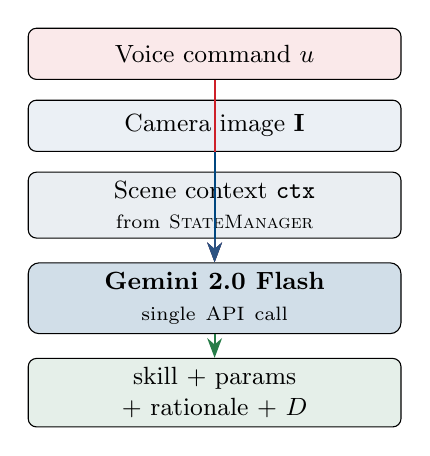
\begin{tikzpicture}[node distance=0.25cm]
        \node[pbox,fill=cRed10] (cmd) {Voice command $u$};
        \node[pbox,fill=cNavy8,below=of cmd] (img)
              {Camera image $\mathbf{I}$};
        \node[pbox,fill=cBlue10,below=of img]
              (ctx) {Scene context \texttt{ctx}\\
                     {\scriptsize from \textsc{StateManager}}};
        \node[draw,rounded corners,fill=cNavy18,
              text width=4.5cm,minimum height=0.9cm,
              align=center,font=\small\bfseries,
              below=0.3cm of ctx] (gem)
              {Gemini 2.0 Flash\\
               {\scriptsize\normalfont single API call}};
        \node[pbox,fill=cGreen12,below=0.3cm of gem]
              (out) {skill + params + rationale + $D$};
        \draw[arr,draw=upecred](cmd)--(gem);
        \draw[arr,draw=navyblue](img)--(gem);
        \draw[arr,draw=softblue](ctx)--(gem);
        \draw[arr,draw=softgreen](gem)--(out);
      \end{tikzpicture}
    \end{column}
  \end{columns}
\end{frame}

% =====================================================================
\section{Semantic World Model}
% =====================================================================

\begin{frame}{\textsc{StateManager} --- Live Semantic Belief State}
  \begin{columns}[T]
    \begin{column}{0.50\textwidth}
      \textbf{Problem:} a cloud VLM is completely
      \emph{stateless} --- it forgets everything between calls.

      \vspace{0.35em}
      \textbf{Solution:} \textsc{StateManager} persists across the session:
      \begin{itemize}\small
        \item Tracks every detected object (bbox, position, count)
        \item Computes spatial relations from bounding boxes automatically
        \item Records gripper state and task history
        \item \textbf{Serialises everything as text prepended to each VLM prompt}
      \end{itemize}

      \vspace{0.3em}
      \begin{alertblock}{Effect}
        \small
        A stateless cloud API becomes a
        \textbf{stateful, session-aware agent.}
      \end{alertblock}
    \end{column}

    \begin{column}{0.46\textwidth}
      \textbf{Context injected into every VLM prompt:}
      \vspace{0.2em}

      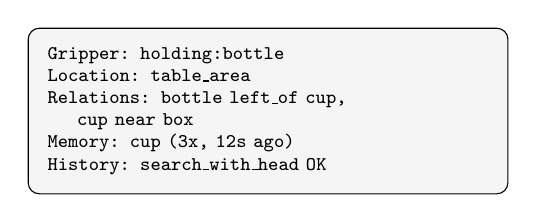
\begin{tikzpicture}
        \node[draw,rounded corners,fill=lightgray,
              text width=5.6cm,font=\ttfamily\scriptsize,
              inner sep=7pt] {
          Gripper: holding:bottle\\
          Location: table\_area\\
          Relations: bottle left\_of cup,\\
          \hspace*{1.1em} cup near box\\
          Memory: cup (3x, 12s ago)\\
          History: search\_with\_head OK
        };
      \end{tikzpicture}

      \vspace{0.35em}
      \begin{exampleblock}{\small Auto spatial relation rules}
        \scriptsize
        \begin{tabular}{ll}
          dist $<$ 150\,px  & \texttt{near}\\
          centroid$_1$ left  & \texttt{left\_of}\\
          bottom edges $\pm$50\,px & \texttt{on\_table}\\
          age $>$ 5\,min & excluded from context\\
        \end{tabular}
      \end{exampleblock}
    \end{column}
  \end{columns}
\end{frame}

% =====================================================================
\section{Grasping Pipeline}
% =====================================================================

\begin{frame}{Active Visual Search}
  \begin{columns}[T]
    \begin{column}{0.54\textwidth}
      \textbf{Problem:} the target object may not be visible
      in the robot's initial field of view.

      \vspace{0.35em}
      \textbf{Solution:} \texttt{search\_with\_head} ---
      systematically scan before attempting any grasp.

      \vspace{0.25em}
      \begin{block}{Scan pattern}
        \begin{itemize}\small
          \item \textbf{12 pan/tilt positions} cover the workspace
          \item Pan: $-1.4$ to $+1.4$\,rad (left/right)
          \item Tilt: $-0.45$ to $+0.3$\,rad (table/shelves)
          \item VLM queries for target at each stop
          \item \textbf{Search ends as soon as target is found}
        \end{itemize}
      \end{block}

      \vspace{0.2em}
      {\small For person targets: face-visibility check prevents
      false positives on feet or torsos.}
    \end{column}

    \begin{column}{0.42\textwidth}
      \centering
      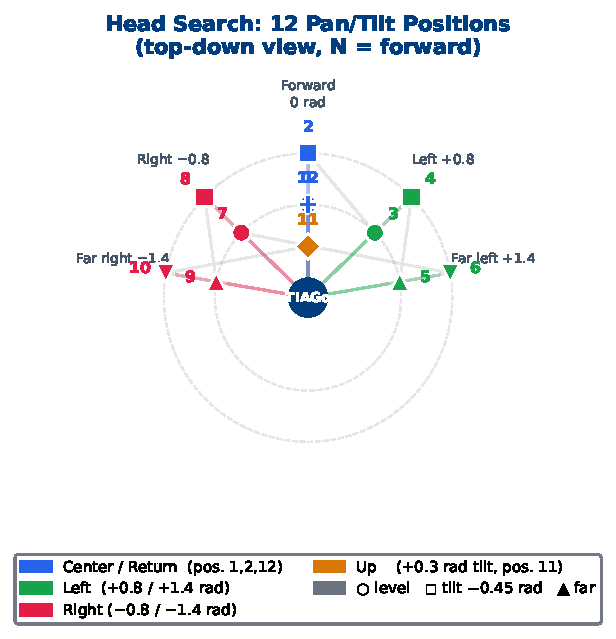
\includegraphics[width=\linewidth,height=0.68\textheight,keepaspectratio]{figs/fig3_headscan.pdf}
    \end{column}
  \end{columns}
\end{frame}

\begin{frame}{Depth-Based Bounding Box Refinement}
  \vspace{-0.2em}
  {\small
  \textbf{Problem:} VLM boxes are semantically correct but spatially coarse
  (include table \& background). Raw box $\Rightarrow$ wrong 3D pose $\Rightarrow$ arm misses.
  \quad\textbf{Fix:} depth-filter to nearest foreground cluster $\pm$\,12\,cm.}

  \vspace{0.3em}
  \begin{center}
    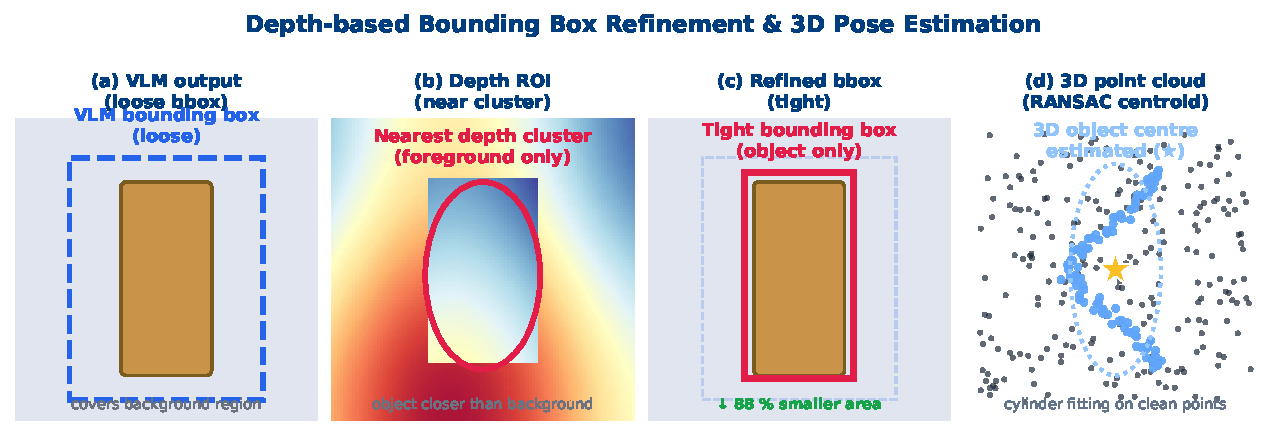
\includegraphics[width=\textwidth,height=0.68\textheight,keepaspectratio]{figs/fig4_depth.pdf}
  \end{center}
\end{frame}

\begin{frame}{3D Pose Estimation and Arm Execution}
  \begin{columns}[T]
    \begin{column}{0.50\textwidth}
      \begin{block}{Pose estimation pipeline}
        \begin{enumerate}\scriptsize
          \item \textbf{Back-projection:} depth + intrinsics
                $(f_x,f_y,c_x,c_y)$ + TF to base frame
          \item \textbf{RANSAC cylinder fit:} centre $(x,y)$
                and radius --- works for bottles and cans
          \item \textbf{Centroid fallback:} median of front-face cluster
                for flat or box-shaped objects
          \item \textbf{Stability:} 5 estimates averaged;
                reachability check removes out-of-reach poses
        \end{enumerate}
      \end{block}

      \vspace{0.05em}
      \begin{block}{Arm execution --- top-down grasp}
        \begin{enumerate}\scriptsize
          \item MoveIt plans collision-free path \textbf{20\,cm above} object
          \item Torso lift joint descends \textbf{straight down}
                (no IK --- guaranteed vertical approach)
          \item Gripper closes; trunk rises; arm goes home
        \end{enumerate}
      \end{block}
    \end{column}

    \begin{column}{0.46\textwidth}
      \centering
      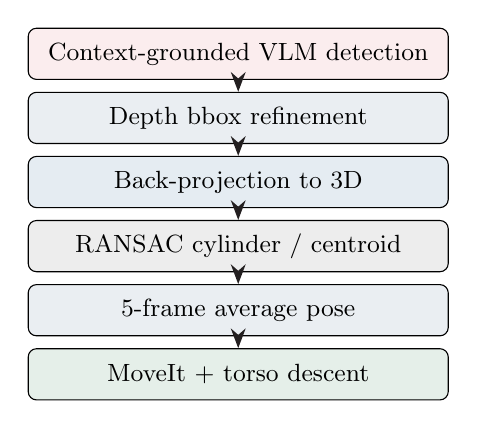
\begin{tikzpicture}[node distance=0.15cm]
        \node[pbox,fill=cRed8,text width=5.1cm]
              (det){Context-grounded VLM detection};
        \node[pbox,fill=cBlue10,text width=5.1cm,below=of det]
              (ref){Depth bbox refinement};
        \node[pbox,fill=cNavy10,text width=5.1cm,below=of ref]
              (bp) {Back-projection to 3D};
        \node[pbox,fill=cDark8,text width=5.1cm,below=of bp]
              (ran){RANSAC cylinder / centroid};
        \node[pbox,fill=cBlue10,text width=5.1cm,below=of ran]
              (avg){5-frame average pose};
        \node[pbox,fill=cGreen12,text width=5.1cm,below=of avg]
              (arm){MoveIt + torso descent};
        \draw[arr,draw=upecdark](det)--(ref);
        \draw[arr,draw=upecdark](ref)--(bp);
        \draw[arr,draw=upecdark](bp)--(ran);
        \draw[arr,draw=upecdark](ran)--(avg);
        \draw[arr,draw=upecdark](avg)--(arm);
      \end{tikzpicture}
      \vspace{0.1em}
      {\scriptsize\color{upecgray} No GPU. No segmentation model.
        Standard laptop CPU.}
    \end{column}
  \end{columns}
\end{frame}

% =====================================================================
\section{Handover \& Face Recognition}
% =====================================================================

\begin{frame}{Handover and Face Recognition}
  \begin{columns}[T]
    \begin{column}{0.50\textwidth}
      \begin{block}{Handover skill}
        \begin{enumerate}\small
          \item Return home; clear stale MoveIt planning scene
          \item VLM detects person in current RGB frame
          \item Depth back-projects person centroid to 3D
          \item MoveIt extends arm at \textbf{0.85\,m height},
                up to \textbf{0.62\,m} toward person
          \item TTS: ``Please take the object from my hand''
          \item Wait \textbf{4\,s} $\to$ open gripper $\to$ go home
        \end{enumerate}
      \end{block}
      \vspace{0.15em}
      {\small Person collision box added during planning ---
       arm cannot hit the person.}
    \end{column}

    \begin{column}{0.46\textwidth}
      \begin{block}{\textsc{FaceManager} --- identity recognition}
        \begin{itemize}\small
          \item Separate HTTP microservice (decoupled from ROS)
          \item Encodes faces as compact embedding vectors
          \item Matches by Euclidean distance below fixed threshold
        \end{itemize}
      \end{block}
      \vspace{0.3em}
      \begin{exampleblock}{Social interaction}
        \begin{itemize}\small
          \item \textbf{Known person} $\to$ robot greets by name
          \item \textbf{Unknown face} $\to$ robot asks name via STT,
                VLM parses response, face stored for session
        \end{itemize}
      \end{exampleblock}
    \end{column}
  \end{columns}
\end{frame}

% =====================================================================
\section{Discussion}
% =====================================================================

\begin{frame}{Key Insights}
  \begin{columns}[T]
    \begin{column}{0.48\textwidth}
      \begin{block}{Neuro-symbolic agent loop}
        \small
        VLM: rich, open-vocabulary observations.\\
        \textsc{SM}: structured, interpretable world model.\\[0.2em]
        Together: stateless cloud API becomes a
        \textbf{stateful, session-aware agent.}
      \end{block}
      \vspace{0.3em}
      \begin{block}{Live vs.\ static ontology}
        \small
        Unlike offline RDF graphs, \textsc{SM} updates
        at every inference step from live detections.\\[0.2em]
        Once an object is grasped, the state change propagates
        immediately --- re-grasping is impossible.
      \end{block}
    \end{column}

    \begin{column}{0.48\textwidth}
      \begin{block}{Unified VLM = lightweight planning}
        \small
        Single model for detection + skill selection
        eliminates the detect-then-plan error cascade.\\[0.2em]
        \texttt{rationale} acts as chain-of-thought seeding the
        grasp-level prompt --- hierarchical planning without
        a separate planner.
      \end{block}
      \vspace{0.3em}
      \begin{alertblock}{Computational footprint}
        \small
        \textbf{No local GPU.} RANSAC, MoveIt, ROS all on
        a standard laptop CPU.\\[0.2em]
        Trade-off: Gemini API outage = system failure.
      \end{alertblock}
    \end{column}
  \end{columns}
\end{frame}

\begin{frame}{Limitations and Future Work}
  \begin{columns}[T]
    \begin{column}{0.48\textwidth}
      \textbf{Current limitations:}
      \begin{itemize}\small
        \item \textbf{Geometry:} RANSAC cylinder fails on flat,
              irregular, or handle-bearing objects
        \item \textbf{Cluttered scenes:} nearest-depth cluster
              can merge adjacent objects at the same depth
        \item \textbf{Cloud dependency:} network outage
              stops the system
        \item \textbf{Static locations:} navigation targets
              hardcoded; no semantic 3D map yet
        \item \textbf{Evaluation:} controlled lab only ---
              unstructured environments not yet tested
      \end{itemize}
    \end{column}

    \begin{column}{0.48\textwidth}
      \textbf{Future directions:}
      \begin{itemize}\small
        \item Superquadric fitting or learned grasp templates
              for non-cylindrical objects
        \item Instance segmentation for cluttered scenes
        \item Local VLM (LLaVA-7B) for offline resilience
        \item SayPlan-style semantic 3D map for multi-room
              deployment
        \item Task-adaptive memory timeout (vs.\ fixed 5\,min)
        \item Structured experiments: success rates,
              ablation of depth refinement vs.\ raw VLM box
      \end{itemize}
    \end{column}
  \end{columns}
\end{frame}

% =====================================================================
\section{Conclusion}
% =====================================================================

\begin{frame}{Conclusion}
  \begin{columns}[T]
    \begin{column}{0.56\textwidth}
      \textbf{What we demonstrated on real TIAGo:}
      \vspace{0.25em}
      \begin{enumerate}\small
        \item \textbf{Closed perception-reasoning-action loop}\\
              Voice command $\to$ physical handover,
              without a GPU
        \item \textbf{Live semantic state injection}\\
              Spatial relations inferred every step;
              multi-instance disambiguation without weight updates
        \item \textbf{Unified VLM} (Gemini 2.0 Flash)\\
              Open-vocabulary detection + skill selection
              in a single API call
        \item \textbf{Depth foreground extraction}\\
              Tight 3D localisation from loose VLM boxes,
              no segmentation model
      \end{enumerate}
      \vspace{0.2em}
      {\small\color{upecgray}
        A practical blueprint for language-guided manipulation
        on commodity service robots.}
    \end{column}

    \begin{column}{0.40\textwidth}
      \centering
      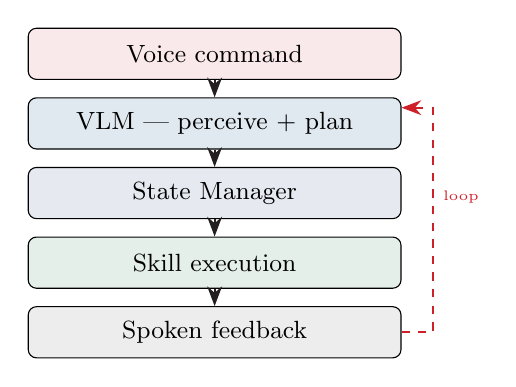
\begin{tikzpicture}[node distance=0.22cm]
        \node[pbox,fill=cRed10] (v) {Voice command};
        \node[pbox,fill=cNavy12,below=of v] (vlm) {VLM --- perceive + plan};
        \node[pbox,fill=cBlue12,below=of vlm] (sm) {State Manager};
        \node[pbox,fill=cGreen12,below=of sm] (sk) {Skill execution};
        \node[pbox,fill=cDark8,below=of sk] (fb) {Spoken feedback};
        \draw[arr,draw=upecdark](v)--(vlm);
        \draw[arr,draw=upecdark](vlm)--(sm);
        \draw[arr,draw=upecdark](sm)--(sk);
        \draw[arr,draw=upecdark](sk)--(fb);
        \draw[arr,draw=upecred,dashed]
          (fb.east)--++(0.4,0)|-([yshift=0.2cm]vlm.east)
          node[pos=0.3,right,font=\tiny,color=upecred]{loop};
      \end{tikzpicture}
      \vspace{0.3em}
      \begin{alertblock}{\centering\small No GPU \enspace No retraining \enspace Real TIAGo}
      \end{alertblock}
    \end{column}
  \end{columns}
  \begin{center}
    \vspace{0.1em}
    \textcolor{upecred}{\rule{0.5\textwidth}{0.8pt}}\\[0.05cm]
    {\scriptsize\color{upecgray}
      LISSI Laboratory --- UPEC --- ECAI 2026 Preprint}
  \end{center}
\end{frame}

% -------------------- THANK YOU --------------------
{
\setbeamertemplate{footline}{}
\begin{frame}
  \begin{center}
    \vspace{1.0cm}
    {\LARGE\bfseries\color{upecdark} Thank You}\\[0.5cm]
    \textcolor{upecred}{\rule{0.45\textwidth}{1.2pt}}\\[0.4cm]
    {\large\color{upecgray} Questions?}\\[0.5cm]
    {\normalsize
      \textbf{Abderrahmene Amar Benhamlaoui}\\[0.15cm]
      LISSI Laboratory ---
      Universit\'{e} Paris-Est Cr\'{e}teil (UPEC)\\[0.15cm]
      \texttt{ferhat.attal@u-pec.fr}}
  \end{center}
\end{frame}
}

\end{document}
